\subsection{Electric Flux}
\hrulefill

\begin{figure}[h]
    \centering
    \begin{subfigure}{0.4\textwidth}
        \centering
        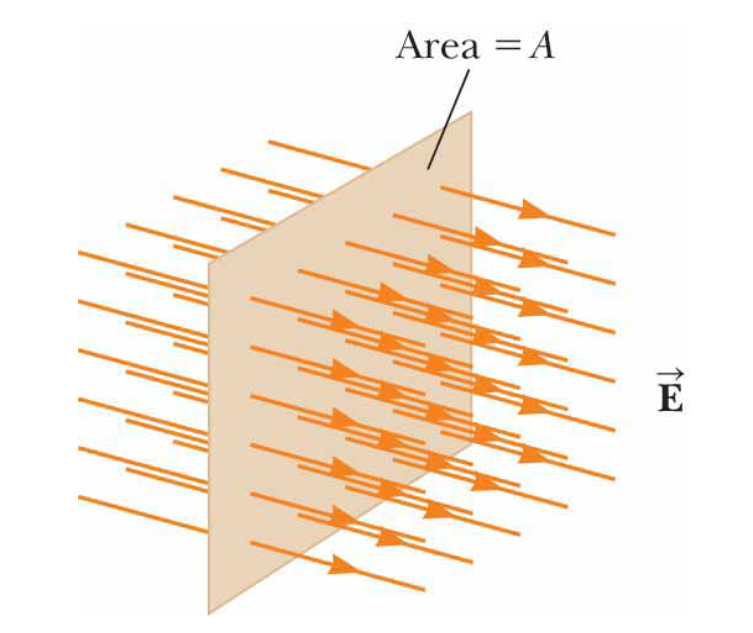
\includegraphics[scale=0.15]{flux.png}
    \end{subfigure}%
    \hspace{0.1\textwidth}
    \begin{subfigure}{0.4\textwidth}
        \centering
        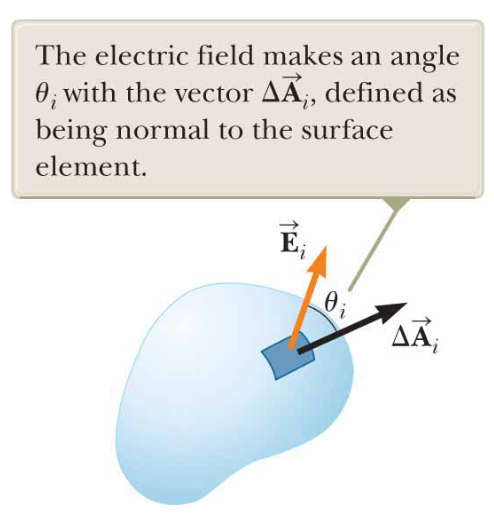
\includegraphics[scale=0.2]{flux1.png}
    \end{subfigure}
\end{figure}

\paragraph*{Definition}
Electric flux is defined as the number of electric field lines passing through a surface. It is measured in Volt meters $[Vm]$.
It is given by the equation:

\begin{equation*}
    \Phi_E = \oint \vec{E} \cdot d\vec{A} = EA\cos(\theta)
\end{equation*}

Where $\Phi_E$ is the electric flux in Newtons per Coulomb, $\vec{E}$ is the electric field in Newtons per Coulomb, $d\vec{A}$ is the differential area vector, and 
$\theta$ is the angle between $\vec{E}$ and $d\vec{A}$.

\hrulefill

\subsubsection*{Gauss's Law}
\paragraph*{Definition}
Gauss's Law states that electric flux through a closed surface is equal to the charge enclosed by the surface divided by the permittivity of free space. This is to say that
any flux generated by electric fields originating from charges outside the surface will cancel out, thus we only care about the enclosed charge.

\begin{equation*}
    \Phi_E = \oint \vec{E} \cdot d\vec{A} = \frac{Q_{\text{enc}}}{\epsilon_0}
\end{equation*}

Where $\Phi_E$ is the electric flux in $Vm$, $\vec{E}$ is the electric field in Newtons per Coulomb, $d\vec{A}$ is the differential area vector, $Q_{\text{enc}}$ 
is the charge enclosed by the surface, and $\epsilon_0$ is the permittivity of free space.